\section{固定基的参数分析}
\label{sec:simplex-parametric}

上一节处理了参数变化之后怎样重新求解。本节问得更早一步：参数在多大范围内变化时，原来的最优基根本不用换，最优解和最优值又怎样随参数变化。

固定最优基$B^\star=(1,5,2)$。式~\eqref{eq:simplex-final-inverse}给出了它的逆矩阵，所有结论都来自这个矩阵。基保持最优需要两个条件：$\bm{x}_B\geq\bm{0}$保证原始可行，$\bm{s}\geq\bm{0}$保证对偶可行。右端变化只影响前者，目标系数变化只影响后者。

\paragraph{右端变化}
设第$i$个资源变化$\delta$，即$\bm{b}(\delta)=\bm{b}+\delta\bm{e}_i$。基不变时，基变量和目标值都是$\delta$的线性函数：
\begin{equation}
 \bm{x}_B(\delta)=\bar{\bm{x}}_B+\delta\,\bm{A}_B^{-1}\bm{e}_i,
 \qquad
 f(\delta)=p^\star+\delta\,y_i.
 \label{eq:simplex-rhs-parametric}
\end{equation}
第二个式子由$f=\bm{b}^\top\bm{y}$和$\bm{y}$不随$\bm{b}$变化得到。基保持可行的条件是$\bm{x}_B(\delta)\geq\bm{0}$，这是对$\delta$的一组线性不等式，解出来是一个区间。

以原料$b_1=8+\delta$为例，$\bm{A}_B^{-1}\bm{e}_1$是式~\eqref{eq:simplex-final-inverse}的第一列，于是
\[
 x_1=4-\frac13\delta,\qquad
 x_5=1-\frac23\delta,\qquad
 x_2=2+\frac23\delta.
\]
三个非负条件分别要求
\[
 \delta\leq12,\qquad \delta\leq\frac32,\qquad \delta\geq-3.
\]
取交集，$\delta\in[-3,3/2]$，也就是$b_1\in[5,9.5]$。图~\ref{fig:simplex-rhs-range}(a)展示了这个范围的几何意义：$b_1$变化时，原料线平行移动，最优顶点沿工时线滑动，下端碰到$x_2=0$，上端碰到设备约束，再走基就要换了。

\begin{BookInlineFigure}
 \centering
 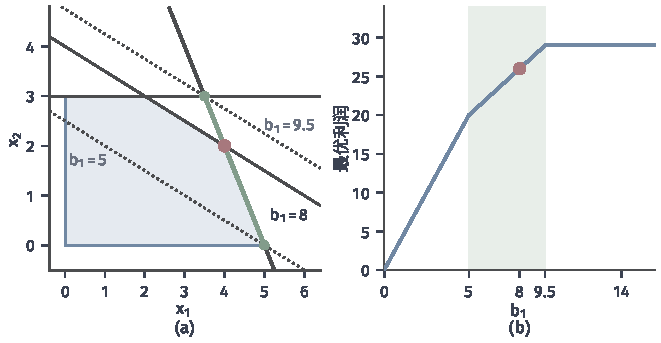
\includegraphics[width=112mm]{figures/05-optimization/01-linear-programming/matplotlib/simplex-rhs-range/figure.pdf}
 \caption{原料$b_1$的有效范围。(a)~实线和点线是$b_1=8$及范围两端$b_1=5,9.5$的原料线，绿色线段是最优顶点随$b_1$滑过的路径，红点是$b_1=8$的最优点。(b)~最优利润随$b_1$的变化（蓝线，对每个$b_1$精确求解），绿色底是基$(1,5,2)$的有效范围，其中斜率恒为影子价格$2$，范围之外斜率改变。}
 \label{fig:simplex-rhs-range}
\end{BookInlineFigure}

\paragraph{影子价格}
在有效范围内，$y_i$就是目标对$b_i$的变化率。按最大化利润的语言，它的相反数是多一单位资源带来的额外利润，称为\term{影子价格}（shadow price）。例中
\[
 -y_1^\star=2,\qquad -y_2^\star=1,\qquad -y_3^\star=0.
\]
一单位原料值$2$，一单位工时值$1$，设备还有富余，增加设备不值钱。如果市场上原料的单价低于$2$，就值得购买，但这个判断只在$b_1\leq9.5$之内有效。超过这个范围，图~\ref{fig:simplex-rhs-range}(b)的斜率变成了$0$，因为此时专用设备成了新的瓶颈。“影子价格”是局部的，它是某个固定基上的数，不是资源的绝对价值。

\paragraph{目标系数变化}
设基变量$x_k$的成本变化$\delta$，$k=B(\ell)$，$\bm{c}(\delta)=\bm{c}+\delta\bm{e}_k$。此时$\bm{x}$不变，对偶候选变化，由式~\eqref{eq:simplex-reduced-cost}计算得到
\begin{equation}
 s_j(\delta)=s_j-\delta\,\bar{a}_{\ell,j}\quad(j\in N),
 \qquad
 f(\delta)=p^\star+\delta\,x_k^\star.
 \label{eq:simplex-cost-parametric}
\end{equation}
其中$\bar{a}_{\ell,j}$是第$\ell$行的系数。基保持最优的条件是$s_j(\delta)\geq0$。若变化的是非基变量$x_j$的成本，只影响它自己的$s_j$，最优基在$s_j+\delta\geq0$时不变。

以产品一的利润为例，$x_1$位于基的第$1$个位置，第$1$行的系数由式~\eqref{eq:simplex-final-inverse}的第一行得到，$\bar{a}_{1,3}=-\frac13$，$\bar{a}_{1,4}=\frac23$。于是
\[
 s_3(\delta)=2+\frac13\delta,\qquad s_4(\delta)=1-\frac23\delta.
\]
非负条件给出$\delta\in[-6,3/2]$。由$c_1=-4+\delta$，换成产品一的利润$p_1=4-\delta$，范围是$p_1\in[2.5,10]$。

图~\ref{fig:simplex-cost-range}说明了这个区间。利润向量转动时，等值线绕最优点转动，最优点保持不动，直到等值线与某条活动约束重合。$p_1=2.5$时利润向量平行于$(1,2)$，$p_1=10$时平行于$(2,1)$，两个端点正好是两条活动约束的法向。

\begin{BookInlineFigure}
 \centering
 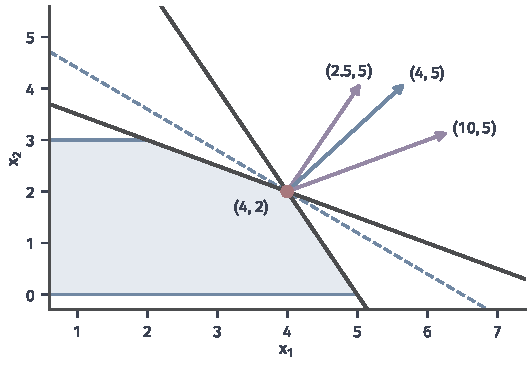
\includegraphics[width=90mm]{figures/05-optimization/01-linear-programming/matplotlib/simplex-cost-range/figure.pdf}
 \caption{产品一利润$p_1$的有效范围。深灰粗线是过$(4,2)$的两条活动约束，蓝色虚线是当前利润$p_1=4$的等值线。三支箭头只表示方向：蓝色是当前利润向量，紫色是范围端点$p_1=2.5$和$p_1=10$的利润向量，两者分别垂直于两条活动约束。}
 \label{fig:simplex-cost-range}
\end{BookInlineFigure}

表~\ref{tab:simplex-parameter-ranges}列出全部五个参数的结果。

\begin{BookInlineTable}
 \centering
 \begin{tabular}{cccl}
  \toprule
  参数 & 当前值 & 有效范围 & 变化率\\
  \midrule
  $b_1$ & $8$ & $[5,\ 9.5]$ & 利润$+2$\\
  $b_2$ & $10$ & $[7,\ 16]$ & 利润$+1$\\
  $b_3$ & $3$ & $[2,\ \infty)$ & 利润不变\\
  $p_1$ & $4$ & $[2.5,\ 10]$ & 利润$+x_1^\star=+4$\\
  $p_2$ & $5$ & $[2,\ 8]$ & 利润$+x_2^\star=+2$\\
  \bottomrule
 \end{tabular}
 \caption{单个参数变化时最优基$(1,5,2)$的有效范围，变化率指参数每增加一单位时最优利润的变化，只在范围内有效。}
 \label{tab:simplex-parameter-ranges}
\end{BookInlineTable}

几个参数同时变化时，结论要从向量形式读取。设右端变化$\Delta\bm{b}$，基$B$保持可行的条件是
\[
 \bar{\bm{x}}_B+\bm{A}_B^{-1}\Delta\bm{b}\geq\bm{0}.
\]
这是$\Delta\bm{b}$的一个多面体，不是逐个区间的乘积。把各个单独的范围同时用到极端，可能已经出界。

\paragraph{越出范围之后}
范围的端点不是答案的终点，只是这个基失效的位置。越过右端的范围，基失去原始可行性而保持对偶可行，这正是第~\ref{sec:simplex-dual}节的出发点。例如$b_1=11$时$x_5=-1$，对偶单纯形法一次换基就得到基$(1,3,2)$和解$(7/2,3)$，利润$29$，这与图~\ref{fig:simplex-rhs-range}(b)的平台一致。

越过目标系数的范围，基失去对偶可行性而保持原始可行，这时用原始单纯形法接着走。例如$p_1=12$时$s_3=-2/3$，$x_3$入基，$\bm{u}=(-1/3,-2/3,2/3)^\top$，比值检验给出$x_2$出基，点走到$(5,0)$，利润$60$。

把一个个基的有效范围拼起来，最优值就成为参数的分段线性函数，图~\ref{fig:simplex-rhs-range}(b)是一个例子，折点是换基发生的位置。在一般约束下，值函数和解映射如何随参数变化，由第~\ref{chap:parametric-sensitivity}章研究。
